% Metódy inžinierskej práce

\documentclass[10pt,twoside,slovak,a4paper]{article}

%%%%%%%%%%%%%%%%%%%%%%%%%%%%%%%%%%%%%%%%%%%%%%%%%%%%%%%%%%%%%%%%%%%%%%%%%%
\usepackage[dvipsnames]{xcolor}
\usepackage[bottom]{footmisc}
\pagenumbering{arabic} %roman - "písmenkové" číslovanie
\usepackage[center]{caption}
\usepackage{footnote}
%%%%%%%%%%%%%%%%%%%%%%%%%%%%%%%%%%%%%%%%%%%%%%%%%%%%%%%%%%%%%%%%%%%%%%%%%%
\usepackage[slovak]{babel}
%\usepackage[T1]{fontenc}
\usepackage[IL2]{fontenc} % lepšia sadzba písmena Ľ než v T1
\usepackage[utf8]{inputenc}
\usepackage{graphicx}
\usepackage{url} % príkaz \url na formátovanie URL
\usepackage{hyperref} % odkazy v texte budú aktívne (pri niektorých triedach dokumentov spôsobuje posun textu)

\usepackage{cite}
%\usepackage{times}

%\pagestyle{headings} %popis v hlavičke - názov nejakej kapitoly a strana hore;	po odstránení je číslo strany dole, ale aj na prvej strane

\title{Vývoj mobilných aplikácií\thanks{Semestrálny projekt v predmete Metódy inžinierskej práce, ak. rok 2021/22, vedenie: Vladimír Mlynarovič}} % meno a priezvisko vyučujúceho na cvičeniach

\author{Lujza Šufliarska\\[2pt]
	{\small Slovenská technická univerzita v Bratislave}\\
	{\small Fakulta informatiky a informačných technológií}\\
	{\small \texttt{xsufliarska@stuba.sk}}
	}

\date{\small 30. september 2021} % upravte



\begin{document}

\maketitle
\thispagestyle{empty} %odstráni z prvej strany číslo strany

\begin{abstract}
\input{abstrakt.txt}
\ldots
\end{abstract}










\section{Úvod}
\quad Témou tohto článku je Vývoj mobilných aplikácií. V niekoľkých kapitolách vám priblížim proces vývoja mobilných aplikácií a pozrieme sa aj na rozdiely pri vývoji aplikácií medzi systémami Android a iOS. Dozviete sa, čo je potrebné urobiť pred začiatkom vývoja, počas, ale aj potom, čo urobíte finálny produkt.



\section{Mobilná aplikácia}
\quad Mobilná aplikácia je softwarová aplikácia vytvorená napríklad pre smartphony a tablety, ktorú je potrebné nainštalovať. Zariadenia sú už vopred vybavené niektorými (základnými) aplikáciami, ale oveľa viac aplikácií (vrátane tých predinštalovaných) je k dispozícii prostredníctvom aplikácie určenej pre ich šírenie – pre systém Android je to aplikácia Obchod Play a pre systém iOS App Store.

Mobilné aplikácie sú určené napr. na produktivitu, navigáciu, komunikáciu, zábavu, šport, fitness a mnoho ďalšieho. V súčasnej dobe máme aplikácie skoro na všetko. Jedným z najpopulárnejších druhov aplikácií sú sociálne siete. Týchto aplikácií je nesmierne veľa a sú tiež najpopulárnejšou oblasťou vývoja.

Načo sú nám mobilné aplikácie, keď existujú webové stránky s rovnakým obsahom? Mobilné aplikácie nám na rozdiel od web stránok ponúkajú väčšiu interaktivitu, konkrétnejšie informácie v jednoduchej a intuitívnej podobe a okrem toho, aplikácia je menšia, prehľadnejšia, pohodlnejšia, ľahšia na prácu, ... ako webová stránka otvorená na mobilnom zariadení.

\cite{eYewated1, eliteml, amazon}



\section{Klasifikácia aplikácií}
\quad Aplikácie vieme rozdeliť do množstva kategórii. Jednou z nich je napríklad rozdelenie podľa vývoja, ktoré je pre nás dôležité. Podľa vývoja vieme aplikácie rozdeliť na \cite{winpc}:
\begin{itemize}
\item  Webové aplikácie

Webové aplikácie sú prístupné cez internet. Tieto aplikácie nepotrebujeme stiahnuť, otvárame ich v prehliadači (Safari, Chrome, Firefox...). Fungujú však len vtedy, keď sme pripojený na internet, a preto sú najmenej praktické.

\item Hybridné aplikácie

Hybridné aplikácie sú kombináciou webovej a natívnej aplikácie. Je možné ich programovať naraz pre obidve platformy. Pri zložitejších funkciách je nutné doprogramovať pre jednotlivé platformy jednotlivé súčasti samostatne. Tento druh aplikácií môže, ale nemusí vyžadovať internetové pripojenie.

\item Natívne aplikácie

Natívne aplikácie sú aplikácie napísané v programovacích jazykoch určených pre iOS alebo pre Android a bežia priamo na operačnom systéme zariadenia. Väčšina mobilných aplikácií je natívnych. Pretože je určená primárne pre jednu platformu, tak sa tento druh aplikácie napr. rýchlejšie inštaluje, ľahšie obsluhuje, nie je závislá od internetového pripojenia, ľahko spolupracuje s funkciami zariadenia... Tento vývoj si však vyžaduje vysoké náklady.

\item Cross-platformové aplikácie

Cross-platformové aplikácie sú vytvorené pre viacero platforiem súčasne. Kód je pre každú platformu skompilovaný do natívnej aplikácie. Tento vývoj môže byť efektívny a menej náročný na zdroje.

\item Progresívne aplikácie

Tento typ aplikácií sa stáva čoraz populárnejším. Aplikácia sa nainštaluje do mobilného zariadenia prostredníctvom prehliadača a nie pomocou obchodu s aplikáciami.
\begin{figure}[h!]
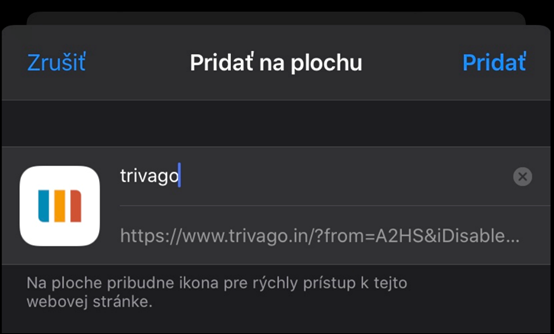
\includegraphics[scale=0.75]{progresivna_aplikacia}
\centering
\caption{Progresívna aplikácia \cite{eliteml}}
\end{figure}

\end{itemize}

\newpage           %ideme na novú stranu


Ďalším veľmi známym rozdelení aplikácií je rozdelenie podľa ich účelu \cite{winpc}:
\begin{itemize}
\item Zábava - hry
\item Pomocníci –počasie, hľadanie informácií...
\item Sociálne siete
\item I-komercia – nákup cez aplikácie
\item ...
\end{itemize}



\section{Proces vývoja aplikácie}
\quad Vývoj mobilných aplikácií je zložitý proces vytvárania aplikácií určených pre mobilné zariadenia. Toto odvetvie je stabilné a výnosné a zaisťuje množstvo pracovných pozícií \cite{eYewated2, wiki1}.

Ako každý vývoj, tak aj vývoj mobilných aplikácií pozostáva z niekoľkých krokov, ktoré tiež závisia od nejakých činiteľov. Nikde nie je presne napísaný postup pre vývoj aplikácií. Ale takou základnou kostrou práce môžu byť tieto body, respektíve fázy \cite{eYewated2, wiki1}:

	\begin{enumerate}
	\item Plán
	\item Grafický návrh aplikácie a prototypovanie
	\item Programovanie aplikácie
	\item Testovanie
	\item Umiestnenie aplikácie na trh
	\item Údržba aplikácie
	\end{enumerate}

\begin{figure}[h!]
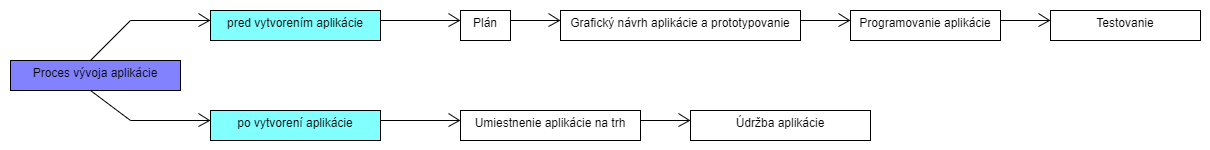
\includegraphics[scale=0.35]{proces_vyvoja_aplikacie}
\caption{Proces vývoja aplikácie
\\ Zdroj: http://www.umletino.com/
\\ Autor: Lujza Šufliarska}
\end{figure}



\subsection{Plán} \label{}
\quad Ešte predtým ako začneme vyvíjať samotnú aplikáciu, treba poznať niekoľko odpovedí na otázky charakterizujúce predstavovanú aplikáciu. Základom k úspešnému projektu je poznať cieľ. Je dobré sa zamyslieť nad niekoľkými otázkami, ako sú napríklad \cite{EMM1, Synetech}:
\begin{itemize}
\item  Čo je zmyslom našej aplikácie?
\item  Je takáto aplikácia potrebná?
\item Aké problémy má aplikácia riešiť?
\item Pre akú cieľovú skupinu má byť aplikácia určená?
\item Aký máme budget?
\end{itemize}


\subsection{Grafický návrh aplikácie}
\quad Teraz prichádza na rad dizajn, kreslenie, storyboarding a wireframing. Najprv si vytvoríme základnú predstavu aplikácie – UI (user interface – užívateľské rozhranie) a UX (user experience) dizajn ( čo je UI a UX je popísané v nasledujúcich podkapitolách).

Na vytvorenie mockupov a screenshotov môžete použiť napr. Adobe XD, Adobe Photoshop, Adobe Illustrator alebo aj Sketch. Storyboard alebo wireframing je podstatnou súčasťou vývoja. Wireframe pretavuje analytickú fázu do grafickej podoby. V priemere sa nakreslí 120 – 150 obrazoviek. Všetky tieto obrazovky a stavy prvkov pomáhajú vo vizualizácií všetkých scenárov.

\begin{figure}[h!]
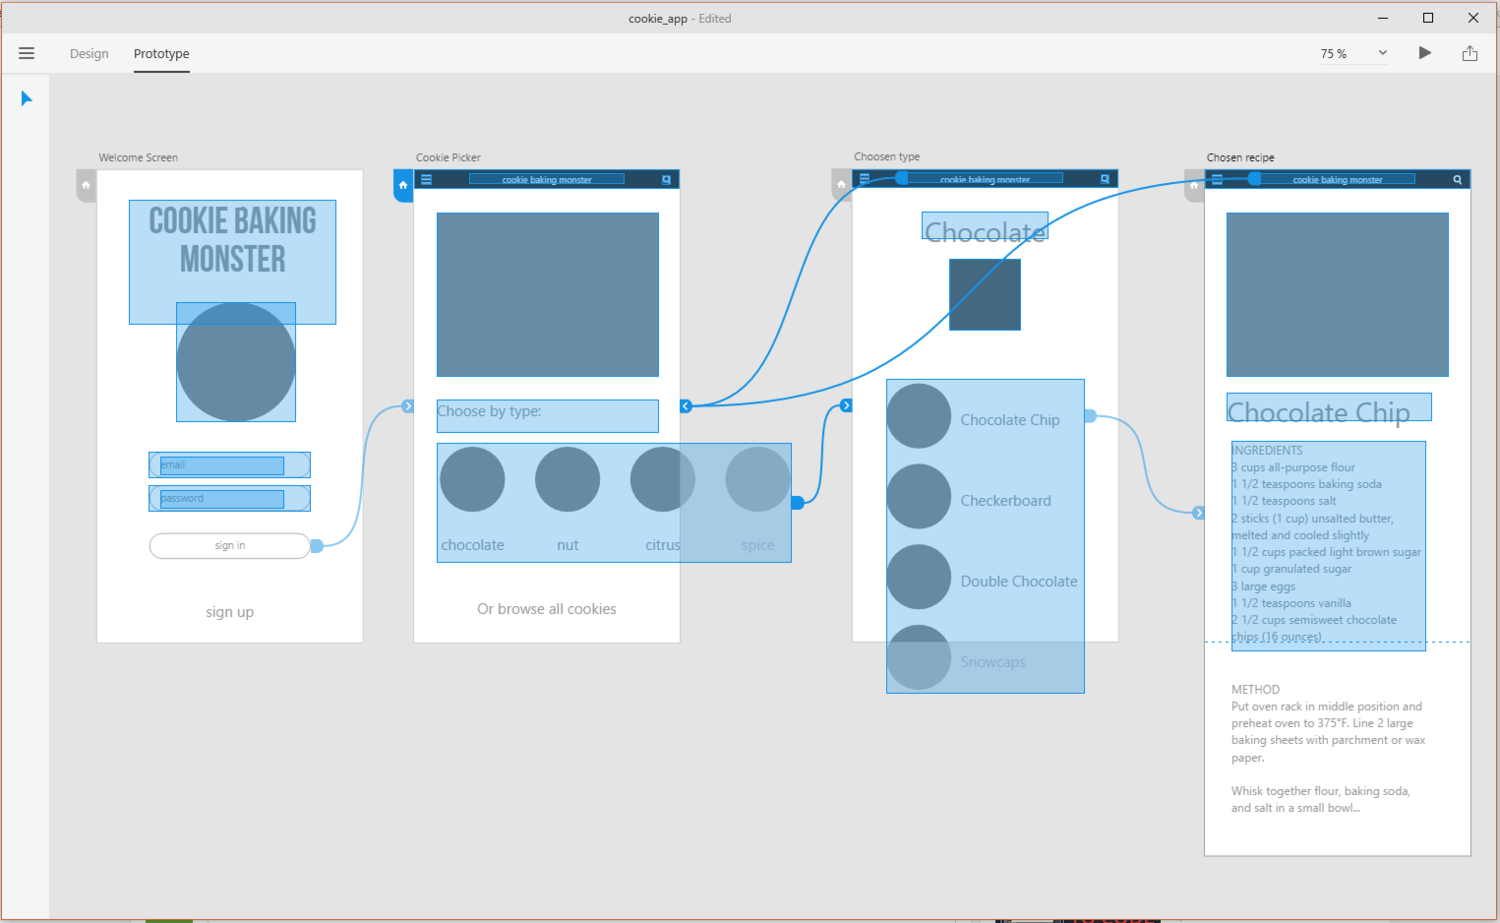
\includegraphics[scale=0.23]{wireframing1}
\centering
\caption{Wireframing
\\ Zdroj: \url{http://www.theresachoi.co/blog/tag/wireframes}}
\end{figure}

\newpage           %ideme na novú stranu

Po navrhnutí wireframov a dizajnu môžeme začať oživovať aplikáciu. Vyrobíme klikateľný prototyp. Opisujeme všetky prechody medzi obrazovkami a stavmi obrazovky, všetky scenáre, animácie... Na to môžeme použiť nástroje Marvel, Flinto, InVision alebo Adobe XD, pomocou ktorých vytvoríme prototyp a uvidíme prvé reakcie a funkcie aplikácie.

\cite{EMM1, winpc}
\\	% vloží prázdny riadok


\textbf{UI}

\quad User interface zahŕňa jednotlivé stránky, podstránky, tlačidlá, vizuále prvky, ktoré pomáhajú pri komunikácii s aplikáciou alebo zariadením. Ide o navrhnutie vizuálne pútavého softvéru a ľahko navigovateľného softvéru pre všetky typy zariadení. Všetky prvky musia byť navrhnuté tak, aby ich úlohy a funkcie boli na prvý pohľad jasné. Tiež musia byť umiestnené na správnych miestach.
\cite{touch4it}
\\	% prázdny riadok


\textbf{UX}

\quad User experience je zážitok, skúsenosť užívateľa po používaní aplikácie alebo webu. Chceme urobiť prepínania medzi jednotlivými podstránkami, stránkami, funkciami urobiť čo najjednoduchšie a intuitívne, aby užívateľ použil náš produkt opakovane a odporučil ho svojim známym. UX zahŕňa aj faktory ako sú dizajn, dostupnosť, marketing, použiteľnosť, výkon systému, užitočnosť...
\cite{touch4it, openxcell}
\\	% prázdny riadok


\textbf{Wireframe}

\quad Wireframe („drôtený model“) pomáha pri návrhu dizajnu, obsahu a funkcií. Väčšinou je to prvá vec,ktorá sa ukazuje klientovi. Prezentuje rozmiestnenie a formu projektu. Definuje textový aj grafický obsah, rozmiestnenie funkčných prvkov, navigáciu, nadpisy, kľúčový text a tlačidlá. Nie je to ale grafický návrh, neobsahuje obrázky, nie sú dôležité farby... Pomocou neho sa vytvorí vzor pre grafikov a vývojárov a použije sa aj na diskusiu s klientom. Robiť zmeny a úpravy je oveľa jednoduchšie a rýchlejšie vo wireframe, ako v hotovom grafickom návrhu alebo naprogramovanej verzii. Wireframe je možné robiť na papier alebo aj v softvéry.
\cite{buildfire, wiki2}

\begin{figure}[h!]
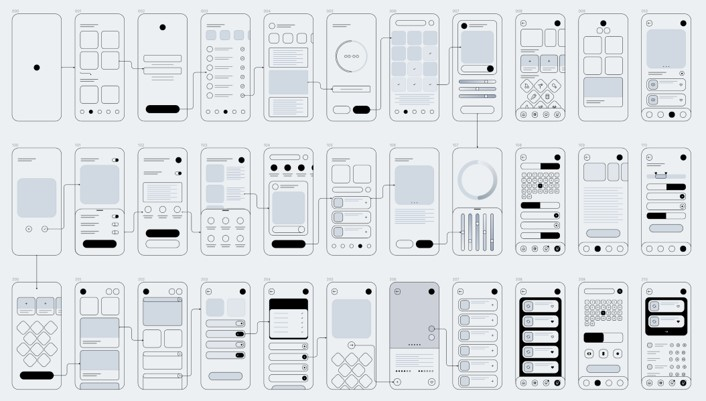
\includegraphics[scale=0.6]{wireframing2}
\centering
\caption{Wireframing
\\ Zdroj: \url{https://www.figma.store/download/wireframes-mobile-free-ui-kit-design-for-figma/}}
\end{figure}


\subsection{Programovanie aplikácie}
\quad Teraz si treba vybrať operačný systém, na ktorom bude aplikácia bežať. Môžeme si vybrať len jeden alebo môžeme vyvinúť cross-platformovú aplikáciu, ktorá najlepšou voľbou. Takto zaistíme, že aplikácia bude fungovať na každom zariadení.
\cite{buildfire}

Väčšinou sa to dá rozdeliť na 3 časti:
\begin{itemize}
\item Back-end vývoj
\item APIs – aplikačné programové rozhranie
\item Front-end vývoj
\end{itemize}



\textbf{Back-end vývoj}

\quad Back-end je vývoj potrebný zo strany servera. Používa sa na uloženie, zaistenie a spracovanie dát. Je to to, čo sa deje, keď užívateľ interaguje s aplikáciou. Dejú sa tu registrácie, prihlásenia, posielanie správ, ukladanie údajov na cloud a mnoho ďalšieho. Back-endový vývoj sa zameriava na ukladanie informácií do vzdialenej databázy, spracovanie vstupu užívateľských dát, skriptovanie na pridanie logiky do interaktivity a vytváranie architektúry, ktorá umožňuje rýchle a jednoduché triedenie informácií. Niektoré aplikácie ako kalkulačka, fotoaparát, kompas nepotrebujú back-endový vývoj, pretože na to, aby fungovali nepotrebujú internetové pripojenie ani ukladanie a obnovovanie údajov a dát zo vzdialeného servera. Ale palikácie ako Amazon, Netflix, Uber nemôžu fungovať bez back-endu.
\cite{openxcell, pixelfield}
\\	% prázdny riadok


\textbf{APIs – aplikačné programové rozhranie}

\quad Application programming interface – API je rozhranie, ktoré definuje spôsoby, ktorými môže aplikácia požadovať služby od knižníc alebo operačných systémov. Aplikácie môžu medzi sebou komunikovať, spoločne pracovať a odosielať si údaje bez toho, aby sa muselo pracovať osobitne s každým programom. Teda umožňuje dvom aplikáciám nájsť sa a vzájomne spolupracovať. Vďaka nemu je rozšírenie alebo napojenie na ďalší systém jednoduché. API pomáha užívateľom rýchlo integrovať a pripojiť sa k vzdialenému cloudovému dátovému serveru. 
\cite{vivantina, wikigis}
\\	% prázdny riadok


\textbf{Front-end vývoj}

\quad Front-end je to čo vidí používateľ. Stará sa o zobrazenie konkrétnych dát, koré sú aplikáciou spracované.

\cite{pixelfield}



\subsection{Testovanie}
\quad Pri testovaní si všímame či sú texty na správnych miestach, či sú funkčné všetky odkazy, tlačidlá a funkcie... Dobrými nástrojmi na testovanie sú napríklad Solidifx alebo Framer. Netreba si myslieť, že keď niečo fungovalo v predchádzajúcich verziách, že to funguje aj vo finálnej verzii. Preto sa treba vrátiť k návrhom a prejsť si všetky funkcie krok za krokom.

Funkčnosť aplikácie je nesmierne dôležitá, preto testujeme na skoro všetkých dostupných zariadeniach. Je dobré testovať aj na modeloch, ktoré dokážu odhaliť množstvo chýb. Väčšinou sú to teda problémové zariadenia, ako napríklad Samsung s5 mini.

\cite{EMM2, buildfire, elite}



\subsection{Umiestnenie aplikácie na trh}
\quad Pred publikovaním aplikácie si treba založiť  účet na Google Play alebo App Store. Vytvorenie účtu môže trvať aj niekoľko dní, a preto na to netreba zabudnúť.

Pri publikácií je dôležité myslieť aj na pravidlá obchodov App Store a Google Play, ktoré sú rozdielne. Napríklad. Google hneď nekontroluje aplikáciu, ale môže to niekedy urobiť. Na druhej strane, Apple ju kontroluje hneď a môže to trvať aj 2 týždne. Existuje aplikácia PreApps, ktorá vám poskytne spätnú väzbu ešte predtým, ako svoju aplikáciu spustíte do obehu.

\begin{figure}[h!]
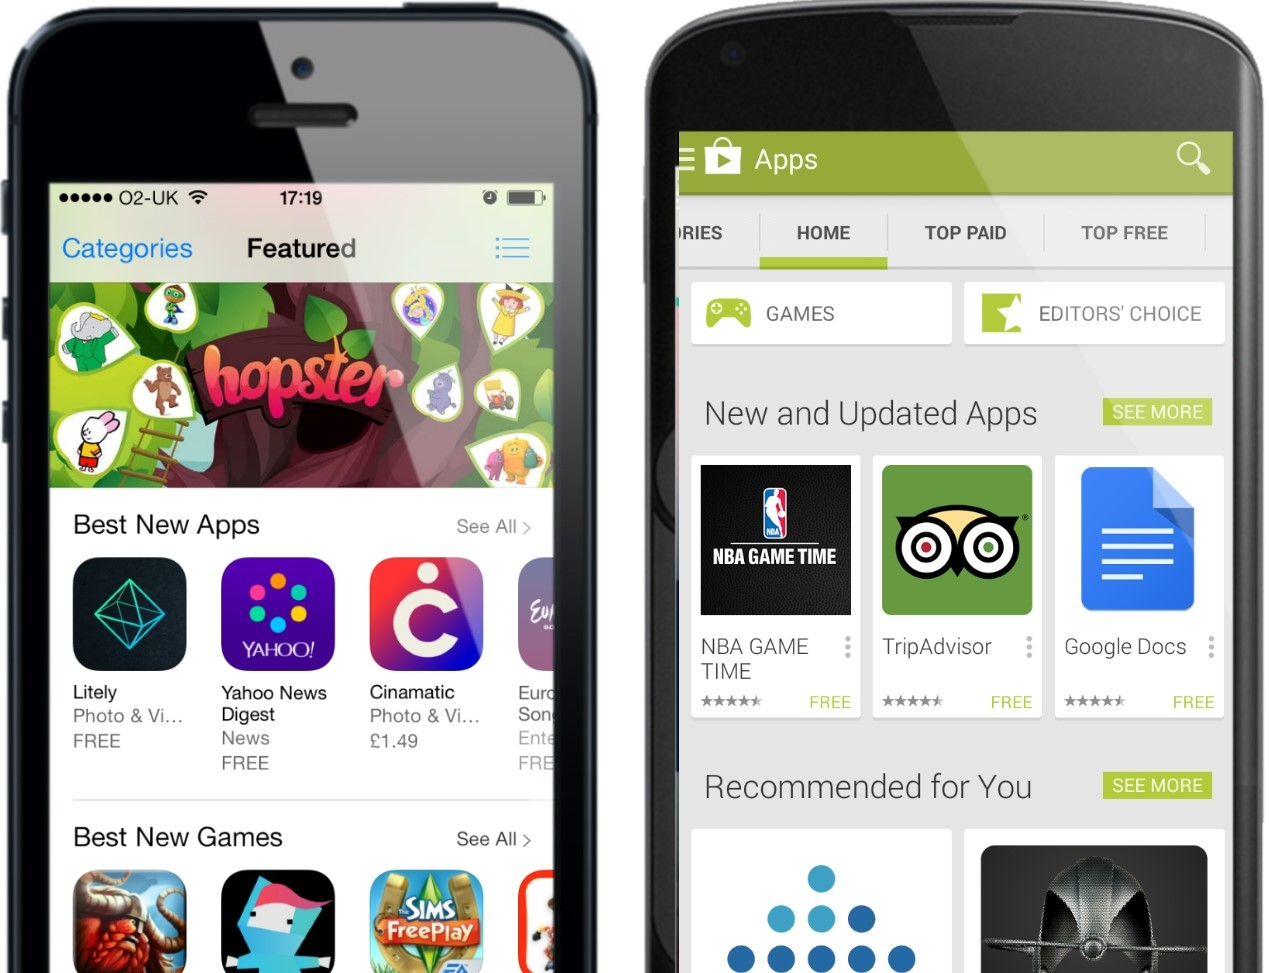
\includegraphics[scale=0.3]{obchod_aplikacii}
\centering
\caption{Obchody aplikácií (App Store naľavo, Google Play napravo) 
\\ Zdroj: \url{https://www.thinkapple.sk/prijmy-app-store-su-2x-vacsie-nez-v-google-play/}}
\end{figure}

\cite{EMM2}

Ak by ste sa chceli dozvedieť viac k tomu, ako umiestniť aplikáciu na trh, odporúčam tieto zdroje (v angličtine):
	\begin{itemize}
	\item pre Android - \url{https://www.youtube.com/watch?v=5GHT4QtotE4} alebo \url{https://appinventiv.com/blog/how-to-submit-app-to-google-play-store/}
	\item pre iOS - \url{https://www.youtube.com/watch?v=YPLs3xrDcm0} alebo \url{https://codewithchris.com/submit-your-app-to-the-app-store/}
	\end{itemize}

\subsection{Údržba aplikácie}
\quad Máte hotovú aplikáciu, ktorú používa niekoľko užívateľov. Ale tu práca nekončí. Aplikáciu treba ďalej udržiavať, optimalizovať, vylepšovať, aby bola stále aktuálna a používaná. Keby sme sa o aplikáciu nestarali, raz by sa zrútila, nefungovala a nakoniec by bola odstránená z obchodu.
\cite{themanifest}



\section{Propagácia aplikácie – pred spustením a po}
\quad Propagácia aplikácie sa dá rozdeliť na propagáciu pred spustením a po. Pred spustením aplikácie sa treba zamerať na vytvorenie záujmu o aplikáciu. Treba poskytnúť všetky dôležité informácie originálnym spracovaním. Dobrým nápadom je spolupracovať s osobami, ktoré majú široký dosah prostredníctvom sociálnych sietí. Môžu si vyskúšať aplikáciu ešte predtým, ako je sprístupnená verejnosti a spropagujú ju cez svoje sociálne siete najlepšie pozitívnou recenziou. Aplikáciu môžete propagovať aj prostredníctvom médií alebo platených článkov. Netreba zabudnúť na zaujímavý popis, informatívne obrázky v obchodoch s aplikáciami a prípadne aj propagačné video.

Po spustení aplikácie sa zamerajte na sociálne siete. Sociálne siete sú najpoužívanejším druhom aplikácií, a preto je najlepším miestom na propagáciu. Pripravte pútavé vizuály, videá a pripojte aj link na stiahnutie aplikácie. Ľudia si skôr stiahnu aplikáciu odporučenú známymi alebo priateľmi. Toto je dobré využiť a poskytnúť odmeny za každého pozvaného užívateľa. Udržujte kontakt. Odpovedajte na otázky a dotazy v obchodoch s aplikáciami. Nezabudnite aj na negatívne komentáre, ktoré vám tiež poskytujú spätnú väzbu. Ako vidíte, je množstvo možností , ako propagovať aplikáciu pred aj po spustení. Stačí si len vybrať, ísť s dobou, aktualizovať propagáciu a teda venovať sa tomu.

\cite{pixelfield}

\begin{figure}[h!]
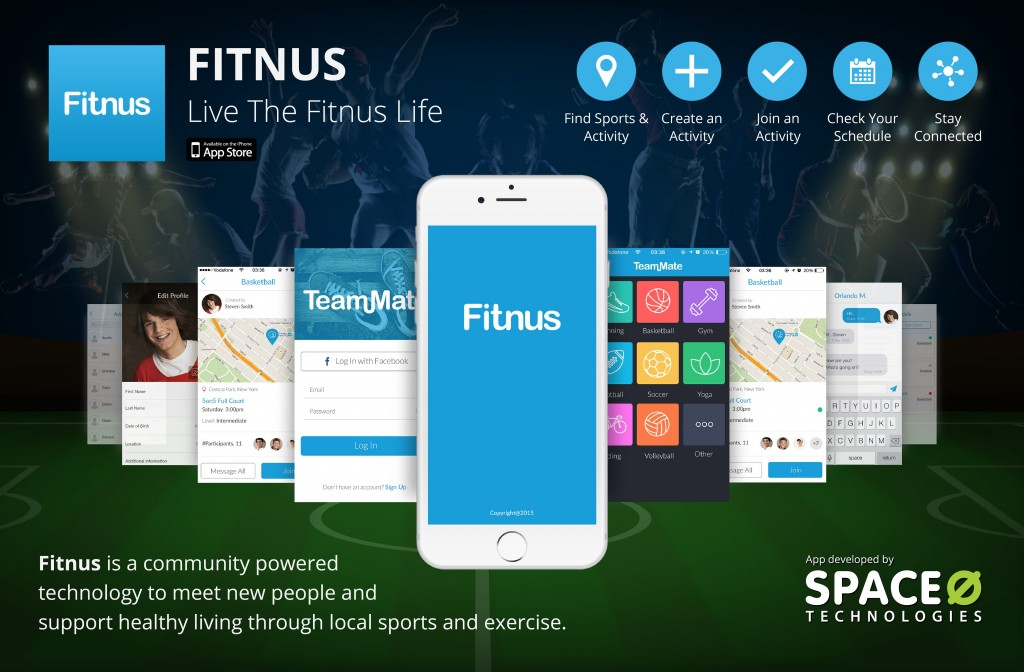
\includegraphics[scale=0.3]{propagacia}
\centering
\caption{Propagácia aplikácie Fitnus
\\ Zdroj: \url{https://www.appfutura.com/blog/add-push-notification-for-android-and-ios-mobile-apps/}}
\end{figure}



\section{Platformy na vývoj aplikácií}
\quad Platformy na vývoj aplikácií sa skladajú z rôznych nástrojov a komponentov, ktoré umožňujú vývojárom písať, testovať a vydávať aplikácie. Medzi platformy na vývoj aplikácií patria napríklad \cite{wiki1, pixelfield}:
\begin{itemize}
\item \textbf{Kotlin} – Tento programovací jazyk sa stal oficiálnym jazykom pre Android. Je možné s ním pracovať napr. vo vývojárskom prostredí Android Studio.
\item \textbf{Swift} – Swift je oficiálnym programovacím jazykom pre iOS aplikácie. Bol vyvinutí spoločnosťou Apple, a aby uľahčil prácu programátorom. Často je používaný XCode ako vývojárske prostredie, ktorý je tiež produktom Apple.
\item \textbf{Flutter} – Umožňuje multiplatformový vývoj. Výslednú aplikáciu je možné zkompilovať do natívneho kódu pre Android aj iOS. Je to mladá technológia, vyvinutá spoločnosťou Google, ktorá používa programovací jazyk Dart 2.
\item \textbf{React Native} – Hybridný framework od Facebooku, ktorý umožňuje písanie aplikácii pre Android aj iOS.
\item \textbf{Apache Cordova} – Jedná sa o ďalší hybridný framework, ktorý je od spoločnosti Apache.
\end{itemize}



\section{Monetizácia aplikácie}
\quad Na to, aby ste mali zisk z aplikácie, nemusí byť aplikácia hneď spoplatnená. Najrozšírenejším spôsobom zárobku sú reklamy. V aplikácii môžete poskytnúť miesta pre reklamu. Tá môže byť spoplatnená napr. na základe počtu kliknutí na ňu. Alebo môžete poskytnúť užívateľom spoplatnenú verziu bez reklám. Ďalším spôsobom je FREEMIUM model. Aplikácia je voľne dostupná, ale má obmedzené funkcie, ktoré majú používateľa tak zaujať, aby si zaplatil plnú verziu PREMIUM so všetkými funkciami. V aplikácii môžete vytvoriť špeciálne predmety, herné vychytávky, doplnkové funkcie... , ktoré si budú môcť užívatelia kúpiť za reálne peniaze. Tento spôsob tvorí až 50\% obratu celého trhu. Takže aj spôsobov, ktorými môžete mať zisk z aplikácie je množstvo. O mnoho viac ako bolo spomenutých.
\cite{pixelfield}

\begin{figure}[h!]
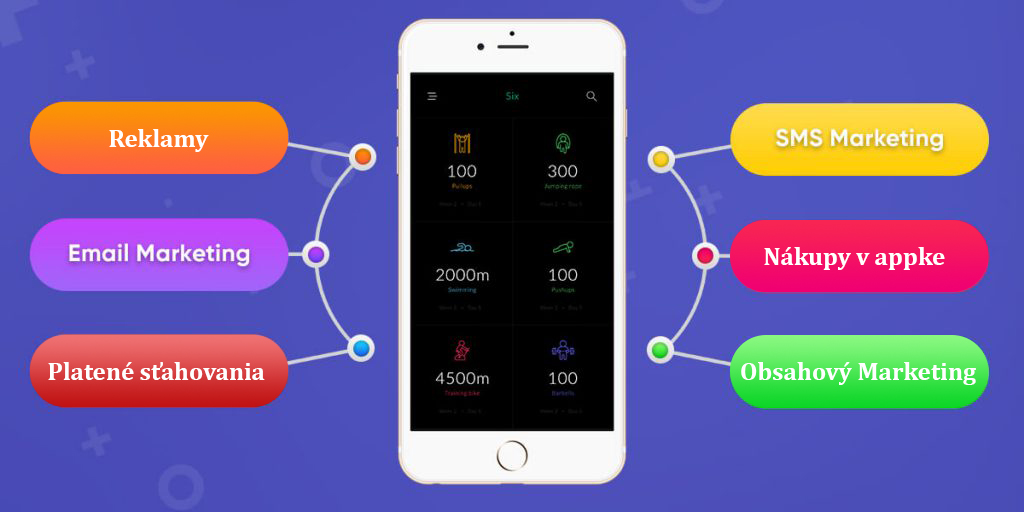
\includegraphics[scale=0.3]{monetizacia}
\centering
\caption{Monetizácia aplikácie
\\ Zdroj: \url{https://www.mindinventory.com/blog/app-monetization-strategies/}
\\ Preklad: Lujza Šufliarska}
\end{figure}



\section{Cena aplikácie}
\quad Ak sme si dali aplikáciu vyrobiť firme, tak nás určite zaujíma aj cena. Cena aplikácie je ovplyvňovaná viacerými faktormi. Medzi ne patrí napríklad dostupnosť aplikácie. To znamená, že na akých zariadeniach bude aplikácia dostupná. Na Android, iOS alebo oboch? Tak isto aj na akých verziách operačného systému bude dostupná. Tu treba dať pozor hlavne na iOS.

Ďalším faktorom je napr. zložitosť a rozsah funkcií. Ideálne je najrpv vytvoriť aplikáciu so základnými funkciami, ku ktorým sa potom pridávajú zložitejšie funkcie, ktoré môžu vývoj predĺžiť a zdražiť.

Dizajn pri mobilných aplikáciách nie je len vzhľad aplikácie, ale aj užívateľské rozhranie (user interface – UI), ale aj funkčnosť a navigácia aplikácie, tzv. user experience – UX.

Veľkosť vývojárskeho tímu tiež ovplyvňuje cenu. Počet členov záleží od zložitosti aplikácie, od požadovaných funkcií. Väčšinou základ tvorí projektový manažér, UX dizajnér, minimálne 2 vývojári a tester. Vo väčšom tíme už nájdeme viacej vývojárov, ktorí sú špecializovaní na určité oblasti – Android, iOS, backend...

Na čom by sa nemalo šetriť je testovanie výslednej verzie aplikácie. Pozorné testovanie môže predísť ďalším nákladom a urýchliť projekt. Ak máme projekt rozdelený na viacej fáz, je dobré po každej fáze všetko otestovať.
Nemôžeme zabudnúť na dlhodobé výdavky na údržbu, úpravu aplikácie, správu dát, vytváranie updateov, poskytovanie podpory užívateľom, výdavky na propagáciu aplikácie...

\cite{pixelfield}



\section{iOS vs. Android vývoj}
\quad Počet užívateľov smartphonov  rastie každým dňom a tak isto narastá aj počet vývojárov aplikácií. V súčasnosti najpoužívanejšími mobilnými operačnými systémami sú iOS, od firmy Apple a Android, od spoločnosti Google. Vývoj aplikácií pre tieto systémy je odlišný a nejaké rozdiely si povieme v tejto kapitole.

\begin{savenotes}
\begin{table}[h!]
\begin{tabular}{|l|l|l|}
\hline
                               & iOS                & Android                      \\ \hline
Programovací jazyk             & Swift, objective-C & Java, Kotlin                 \\ \hline
IDE (vývojové prostredie)      & Xcode              & Android Srudio               \\ \hline
Cena registrácie do obchodu    & \$\begin{math}99\end{math} ročne         & \$\begin{math}25\end{math} jednorázovo             \\ \hline
Schválenie aplikácie v obchode\footnote{tiež spomenuté v kapitole Umiestnenie aplikácie na trh} & V priemere 2 dni   & Krátka doba (niekoľko hodín) \\ \hline
\end{tabular}
\caption{Tabuľka porovnania rozdielov medzi systémami iOS a Android vo vývoji aplikácií}
\end{table}
\end{savenotes}

\textbf{Programovací jazyk}

Na vývoj aplikácii pre systém Android sa používa hlavne programovací jazyk Java, vďaka ktorému je vývoj pre tento systém jednoduchší, pretože je používaný väčšinou vývojárov. Ďalšie programovacie jazyky, ktoré sa môžu použiť na vývoj Android aplikácie sú napríklad Kotlin, Flutter a React Native.

Na aplikácie pre iOS sa v súčasnej dobe používa hlavne Swift. Jeho výhodou je, že je stručný a jednoduchší ako objective-C, ktorý sa tiež používa na vývoj. Objective-C je exkluzívnejšie, čo môže byť prekážkou pre vývojárov menej kvalifikovaných v iných programovacích jazykoch. Okrem týchto jazykov je tiež možné použiť napríklad Flutter alebo React Native.


\cite{eYewated2, openxcell, W2S, appleglitz}
\\	%prázdny riadok


\textbf{IDE (vývojové prostredie)}

Pre vývoj android aplikácii je v súčasnosti najpoužívanejšie Android Studio od Google. Umožňuje cross-platformový vývoj, ladenie aplikácie, úpravu kódu, testovanie, testovanie aplikácie v emulátore (nie je potrebné mať android zariadenie, ale treba rátať s tým, že emulátor nemusí vždy fungovať správne)... Android Studio je možné používať zadarmo na systémoch Windows, macOS aj Linux.

IOS vývojári používajú XCode od Apple pre vývoj iOS aplikácii. Je to rýchly a spoľahlivý softvér. Umožňuje návrh, vývoj, zápis kódu, riešenie problémov, testovanie, dokáže zistiť chyby a errory v syntaxi a logike, dokáže opraviť kód a dokonca umožňuje pridanie aplikácie priamo do obchodu. Xcode je bezplatný program, ale je možné ho používať len na notebookoch a počítačoch Apple. Sú aj nejaké iné možnosti ako vyvíjať Apple aplikácie, ktoré sú spomenuté v tomto článku - \url{https://codewithchris.com/xcode-for-windows/}.

\cite{eliteml, EGO, DDI}

Samozrejme neexistuje len Android Studio a Xcode. Existuje množstvo programov, v ktorých je možné vyvíjať aplikácie pre Android alebo iOS. Android Studio a Xcode sú len najpoužívanejšími aplikáciami.
\\	%prázdny riadok

%pokus o danie obrázkov vedľa seba, ale sú príliž veľké tak sú pod sebou
\begin{figure}[h!]
	\centering
	\begin{minipage}[b]{1\textwidth}
		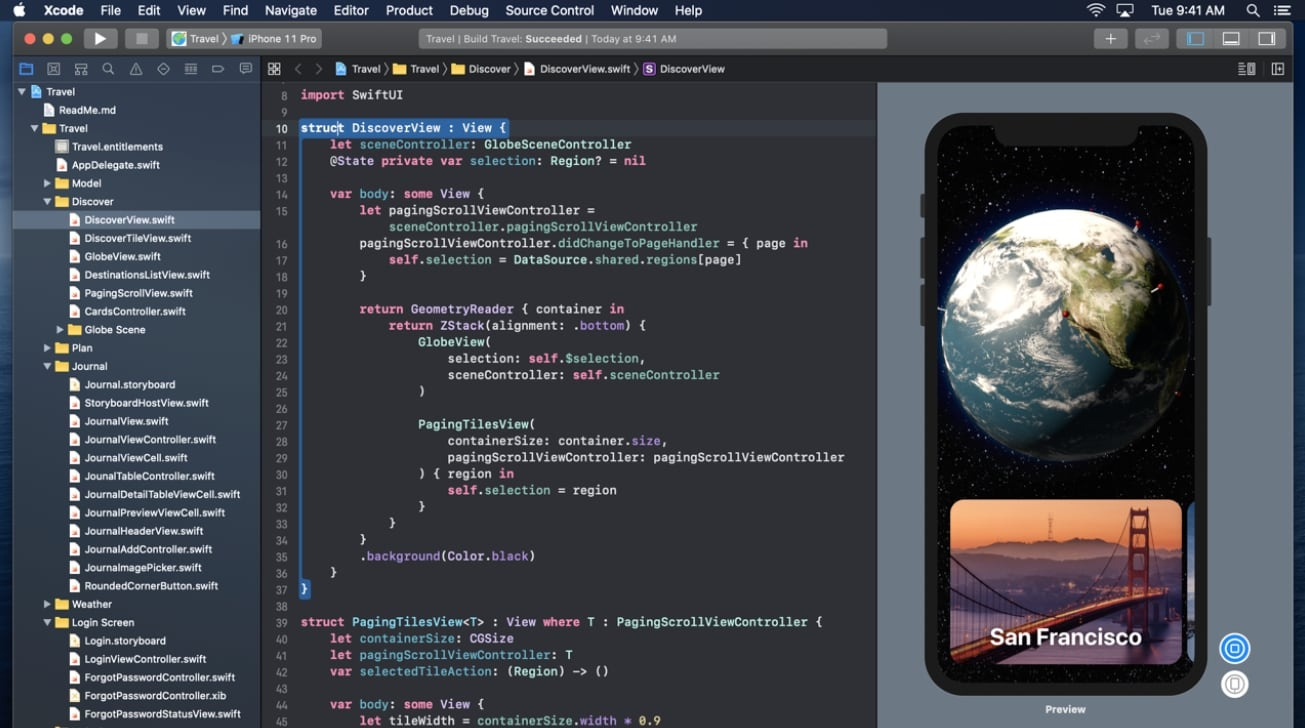
\includegraphics[width=\textwidth]{XCode}
		\caption{Program XCode \cite{appleinsider}}
	\end{minipage}
	\hfill
	\begin{minipage}[b]{1\textwidth}
		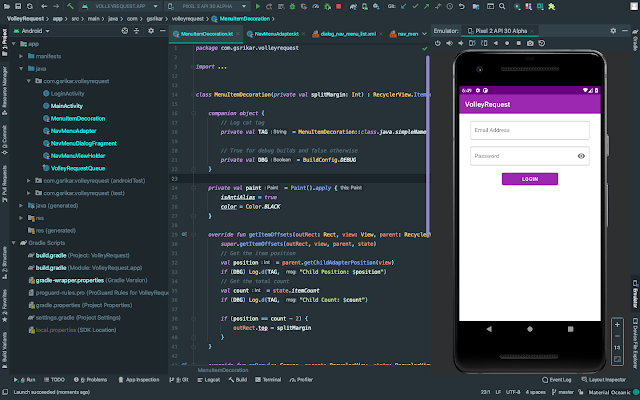
\includegraphics[width=\textwidth]{Android_Studio}
		\caption{Program Android Studio \cite{gStrikar}}
	\end{minipage}
\end{figure}

\newpage           %ideme na novú stranu




\textbf{Platba za registráciu do obchodu}

Pre pridanie aplikácie do obchodu Google Play je potrebné uhradiť jednorázový registračný poplatok \$25. Tento jednorázový poplatok je za registráciu do Google Play Developer Console.
\cite{RedBytes}

Apple App Store si účtuje až \$99 ročne za to, aby mohla byť aplikácia pridaná do obchodu. Tých \$99 je za registráciu (a používanie) do programu Apple Developer Program. Tento progrm vám poskytne prístup k množstvu výhod, ako napríklad pridávanie aplikácií do App Storeu, pridávanie Safari rozšírení, testovacie nástroje, analýza aplikácií....
\cite{CWC}

\cite{RedBytes, eYewated3, eliteml}
\\	%prázdny riadok


\textbf{Schválenie aplikácie}

Schválenie aplikácie v Apple App Store trvalo 3-4 týždne. V súčasnosti je to v priemere 2 dni. Trvá to tak dlho, pretože aplikáciu schvaľuje tím developerov, ktorý prechádza celou aplikáciou, aby odhalil všetky chyby a upozornil na ne autora.

Proces schvaľovania android aplikácie trvá len niekoľko hodín. Aplikáciu kontroluje tím odborníkov pomocou automatizovaných nástrojov. Tím hľadá v aplikácii porušenia, prítomnosť malwareu, spywareu, porušenie autorských práv... Po kontrole prvým tímom, aplikáciu skontroluje ešte druhý tím, ktorý aplikáciu zhodnotí. Keďže nemá Android Market takú prísnu kontrolu, na Google Play sa nachádza veľké množstvo nekvalitných aplikácií.

\cite{eYew3, DZone}
\\	%prázdny riadok


\textbf{Zhrnutie}

Aj Android aj Apple majú svoje plusy aj mínusy. Je ale odporúčané vyvíjať aplikácie aj pre iOS, aj pre Android. Okrem toho, aplikácia dostupná len pre jeden operačný systém pôsobí neprofesionálne a zbytočne prichádza o množstvo potencionálnych zákazníkov.



\section{Záver} \label{zaver} % prípadne iný variant názvu
\quad Po prečítaní tohto článku sme sa dozvedeli, že vyvinúť aplikáciu nie je až také jednoduché. Je to proces, ktorý trvá nejakú dobu. Hlavne, ak chceme vyvinúť poriadnu, funkčnú a spoľahlivú aplikáciu.

Je dôležité urobiť si plán a držať sa ho. Tak si môžeme byť istý, že na nič nezabudneme. Povedali a opísali sme si pár dôležitých krokov pri vývoji, takže predstaviť si a začať vyvíjať aplikáciu by malo byť o niečo jednoduchšie. Vývoj sa dá rozdeliť na 2 časti: na vývoj pred finálnou aplikáciou a na vývoj po finálnej aplikácii. Obidve tieto časti sme si popísali. Dozvedeli sme sa aj niekoľkých možnostiach zisku z aplikácie. Nezabudli sme spomenúť, od čoho závisí cena vývoja aplikácie v prípade, že by sme ju nechceli vyvíjať sami, ale dali by sme si ju vyvinúť napríklad nejakej firme. Ďalej sme si povedali pár rozdielov vo vývoji pre systém Android a iOS. Ako ste mohli vidieť, rozdiely spočívajú hlavne  v programovacom jazyku, vývojovom prostredí a ďalších aspektoch, ktoré sa týkajú hlavne fázy, kedy už máme finálnu aplikáciu.




\section{Reakcia na témy}
spoločenské súvislosti informatiky – označenie: \paragraph{Spoločenské súvislosti.}
história informatiky – označenie: \paragraph{Historické súvislosti.}
technológia a ľudia – označenie: \paragraph{Technológia a ľudia.}
udržateľnosť a etika – označenie: \paragraph{Udržateľnosť a etika.}



%\bibliography{literatura.bib}
%\acknowledgement{Ak niekomu chcete poďakovať\ldots}


% týmto sa generuje zoznam literatúry z obsahu súboru literatura.bib podľa toho, na čo sa v článku odkazujete
\bibliography{literatura}
\bibliographystyle{plain} % prípadne alpha, abbrv alebo hociktorý iný
\end{document}
